\documentclass[10pt]{article}
\usepackage{tikz}
\usetikzlibrary{shapes.misc}
\usepackage[margin=0cm]{geometry}
\pagestyle{empty}
\tikzstyle{every node}=[cross out, draw, red]

\begin{document}

\vspace*{\fill}
\begin{center}
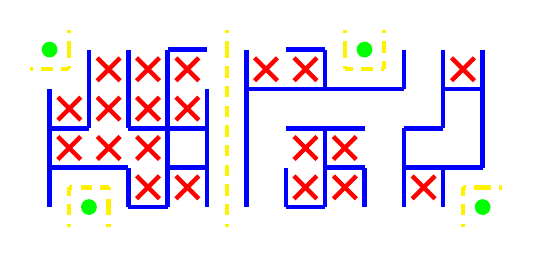
\begin{tikzpicture}[x=0.25cm, y=-0.25cm, ultra thick, blue]
% Walls
	\draw (3,1) -- (3,3);
	\draw (3,3) -- (3,5);
	\draw (1,5) -- (3,5);
	\draw (1,5) -- (1,7);
	\draw (1,3) -- (1,5);
	\draw (1,7) -- (3,7);
	\draw (1,7) -- (1,9);
	\draw (3,7) -- (5,7);
	\draw (5,7) -- (5,9);
	\draw (5,9) -- (7,9);
	\draw (7,7) -- (9,7);
	\draw (7,7) -- (7,9);
	\draw (7,5) -- (9,5);
	\draw (7,5) -- (7,7);
	\draw (7,3) -- (7,5);
	\draw (7,1) -- (9,1);
	\draw (7,1) -- (7,3);
	\draw (9,5) -- (9,7);
	\draw (9,3) -- (9,5);
	\draw (9,7) -- (9,9);
	\draw (5,5) -- (7,5);
	\draw (5,3) -- (5,5);
	\draw (5,1) -- (5,3);
	\draw (11,1) -- (11,3);
	\draw (11,3) -- (13,3);
	\draw (11,3) -- (11,5);
	\draw (13,3) -- (15,3);
	\draw (15,3) -- (17,3);
	\draw (15,1) -- (15,3);
	\draw (13,1) -- (15,1);
	\draw (17,3) -- (19,3);
	\draw (19,1) -- (19,3);
	\draw (11,5) -- (11,7);
	\draw (11,7) -- (11,9);
	\draw (21,1) -- (21,3);
	\draw (21,3) -- (23,3);
	\draw (21,3) -- (21,5);
	\draw (23,3) -- (23,5);
	\draw (23,1) -- (23,3);
	\draw (23,5) -- (23,7);
	\draw (21,7) -- (23,7);
	\draw (21,7) -- (21,9);
	\draw (19,7) -- (21,7);
	\draw (19,7) -- (19,9);
	\draw (19,5) -- (21,5);
	\draw (19,5) -- (19,7);
	\draw (13,5) -- (15,5);
	\draw (15,5) -- (17,5);
	\draw (15,5) -- (15,7);
	\draw (15,7) -- (17,7);
	\draw (15,7) -- (15,9);
	\draw (17,7) -- (17,9);
	\draw (13,9) -- (15,9);
	\draw (13,7) -- (13,9);
% Pillars
	\fill[green] (1,1) circle(0.4);
	\fill[green] (17,1) circle(0.4);
	\fill[green] (3,9) circle(0.4);
	\fill[green] (23,9) circle(0.4);
% Inner points in accessible cul-de-sacs
	\node at (4,2) {};
	\node at (4,4) {};
	\node at (4,6) {};
	\node at (6,6) {};
	\node at (6,8) {};
	\node at (2,6) {};
	\node at (6,2) {};
	\node at (6,4) {};
	\node at (12,2) {};
	\node at (14,2) {};
	\node at (22,2) {};
	\node at (8,2) {};
	\node at (8,4) {};
	\node at (2,4) {};
	\node at (14,6) {};
	\node at (14,8) {};
	\node at (16,6) {};
	\node at (8,8) {};
	\node at (16,8) {};
	\node at (20,8) {};
% Entry-exit paths without intersections
	\draw[dashed, yellow] (2,1) -- (2,0);
	\draw[dashed, yellow] (2,1) -- (2,2);
	\draw[dashed, yellow] (2,2) -- (1,2);
	\draw[dashed, yellow] (1,2) -- (0,2);
	\draw[dashed, yellow] (10,1) -- (10,0);
	\draw[dashed, yellow] (10,1) -- (10,2);
	\draw[dashed, yellow] (10,2) -- (10,3);
	\draw[dashed, yellow] (10,3) -- (10,4);
	\draw[dashed, yellow] (10,4) -- (10,5);
	\draw[dashed, yellow] (10,5) -- (10,6);
	\draw[dashed, yellow] (10,6) -- (10,7);
	\draw[dashed, yellow] (10,7) -- (10,8);
	\draw[dashed, yellow] (10,8) -- (10,9);
	\draw[dashed, yellow] (10,9) -- (10,10);
	\draw[dashed, yellow] (16,1) -- (16,0);
	\draw[dashed, yellow] (16,1) -- (16,2);
	\draw[dashed, yellow] (16,2) -- (17,2);
	\draw[dashed, yellow] (17,2) -- (18,2);
	\draw[dashed, yellow] (18,2) -- (18,1);
	\draw[dashed, yellow] (18,1) -- (18,0);
	\draw[dashed, yellow] (4,9) -- (4,10);
	\draw[dashed, yellow] (4,9) -- (4,8);
	\draw[dashed, yellow] (4,8) -- (3,8);
	\draw[dashed, yellow] (3,8) -- (2,8);
	\draw[dashed, yellow] (2,8) -- (2,9);
	\draw[dashed, yellow] (2,9) -- (2,10);
	\draw[dashed, yellow] (23,8) -- (24,8);
	\draw[dashed, yellow] (23,8) -- (22,8);
	\draw[dashed, yellow] (22,8) -- (22,9);
	\draw[dashed, yellow] (22,9) -- (22,10);
\end{tikzpicture}
\end{center}
\vspace*{\fill}

\end{document}